\chapter{Preliminary concepts}

\todo[inline]{TODO: Find better images}

\section{The central dogma of molecular biology}

The central dogma explains how genetic information flows within a living being. It states that DNA, the molecule that stores the genetic information, is replicated by the enzyme DNA Polymerase. Also, RNA Polymerase produces messenger RNA (mRNA) from DNA in a process called transcription. Finally, the ribosome build the proteins following the sequence of the mRNA and according to a genetic code that translates from the language of nucleotides (the structural blocks of DNA and RNA) to the language of aminoacids, the structural blocks of proteins \cite{alberts13}.

Proteins are the structural and functional elementary units of living beings. Therefore, according to the proteins that are being produced in a certain cell it will develop certain functions. The central dogma is summarized in fig. \ref{fig:con-dogma}.

\begin{figure}[H]
  \centering
  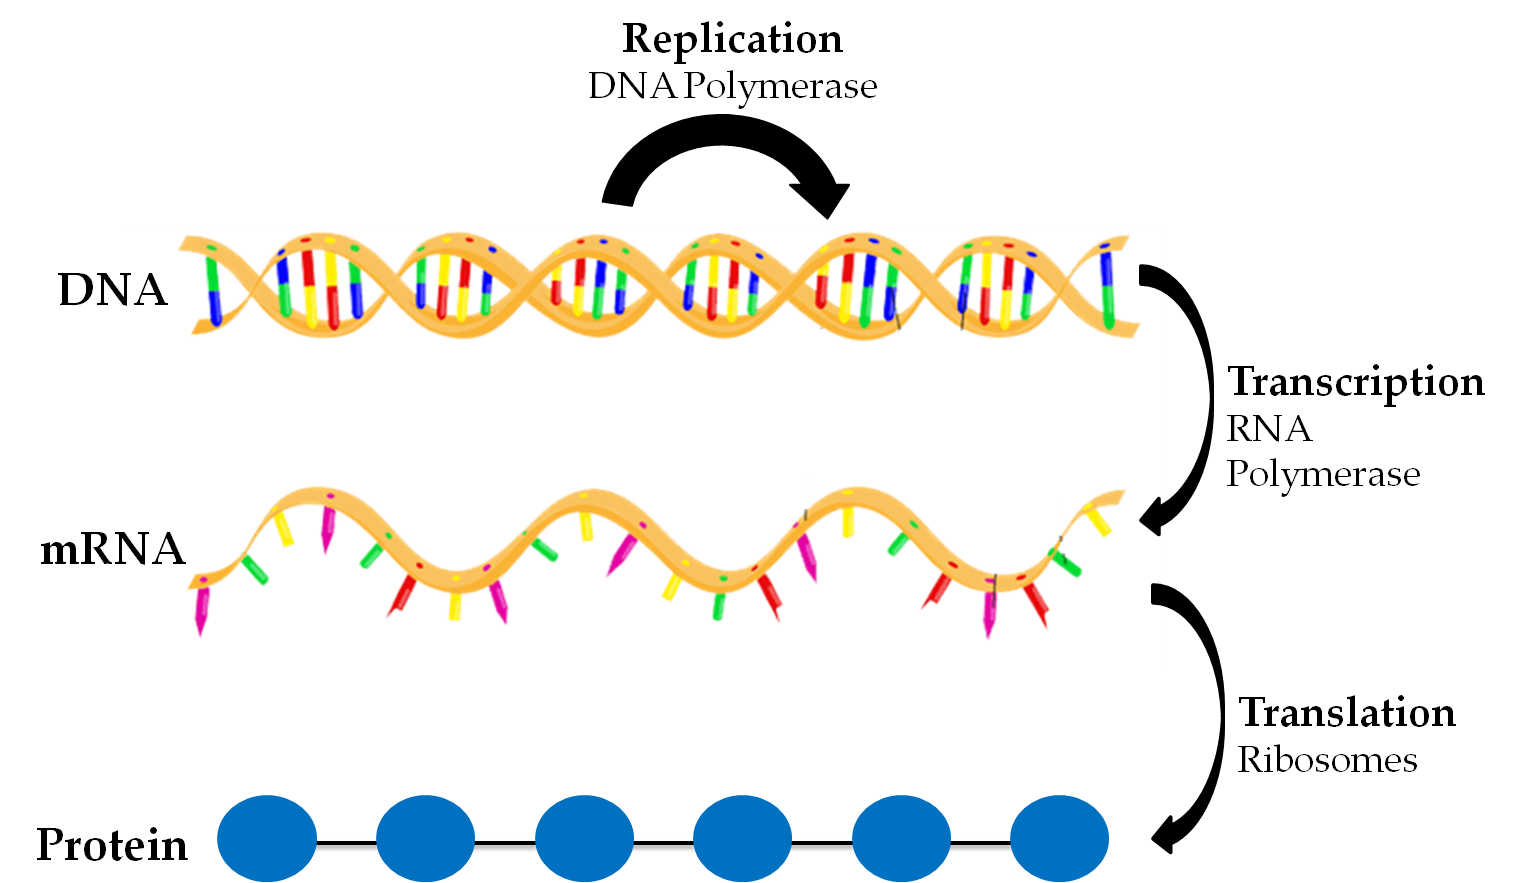
\includegraphics[width=5cm]{con-dogma}
  \caption[Central dogma of molecular biology]{\label{fig:con-dogma} Scheme of the central dogma of molecular biology. By Dhorspool at en.wikipedia, CC BY-SA 3.0, \$3.}
\end{figure}

An important fact is that the central dogma is valid for all the living beings. The encoding of information in DNA and the mechanisms by which proteins are made according to that information, including the genetic code, are very similar between different organisms.

\section{Gene regulation and biological circuits}

DNA contains all the information necessary to build a living being and let him develop his functions. But genetically identical cells may differ a lot. For example, our neurons are very different in form and function than our skin cells, even though they have the same DNA and thus the same genetic information. This differentiation happens because they are expressing different sets of genes. The genetic information encoded in the DNA is called genotype, while the observable characteristics of an organism are called phenotype. In this terminology, both kinds of cells have the same genotype but differ in their genotypes \cite{alberts13} \cite{alon06}.

Those differences lie on the genes that each cell is expressing at a certain time and how much they are being expressed (measured in the rate of production of proteins corresponding to a gene). There are proteins (and even RNA molecules) that inhibit the production of other protein by stoping transcription of the corresponding gene. On the contrary, there are proteins that enhance the production of other proteins by increasing the rate of transcription. Both activators and inhibitors are called \textit{transcription factors}, both cases can be seen on fig. \ref{fig:con-tf_simple}.

\begin{figure}[H]
  \centering
  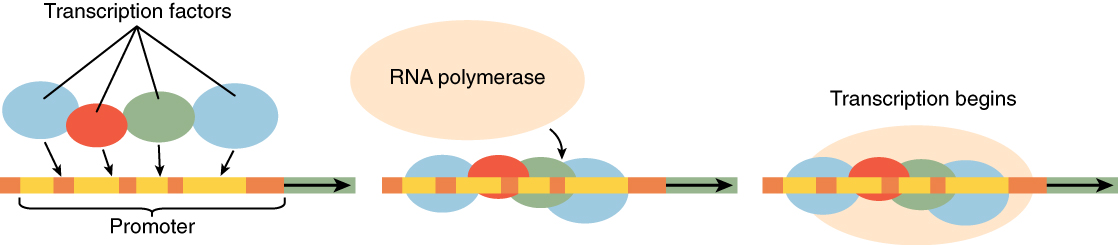
\includegraphics[width=12cm]{con-tf_simple}
  \caption[Transcription factors]{\label{fig:con-tf_simple} Scheme of the mechanisms of transcription factors. Retrieved from: \url{http://biowiki.ucdavis.edu}}
\end{figure}

The mechanisms of gene regulation can be very complex. For example, a molecule can change the conformation of another protein that when affected by the first, inhibits the transcription of certain gene. Those molecules may be signals from the environment and with mechanisms of this type, the cell process environmental signals to express the optimal genes according to the environment. It is also important to point out that the inhibition and activation is not necessarily done individually. A certain gene may need more than one different protein to enhance its activity, or there may be genes that are activated by a protein and inhibited by others, whose production is in turn mediated by other molecules and transcription factors, a well studied case is the \textit{lac} operon in \textit{E. coli} whose mechanism is explained on fig. \ref{fig:con-lac_operon}.

From the biochemical point of view, transcription factors bind specific sites on the \textit{promoter}, a region of the DNA which is upstream the gene (or set of genes for prokaryotes), and it is where the RNA Polymerase binds to initiate transcription (see fig. \ref{fig:con-parts_of_DNA}). The binding of the transcription factor may enhance or obstruct the binding of RNA Polymerase to the promoter.

\begin{figure}[H]
  \centering
  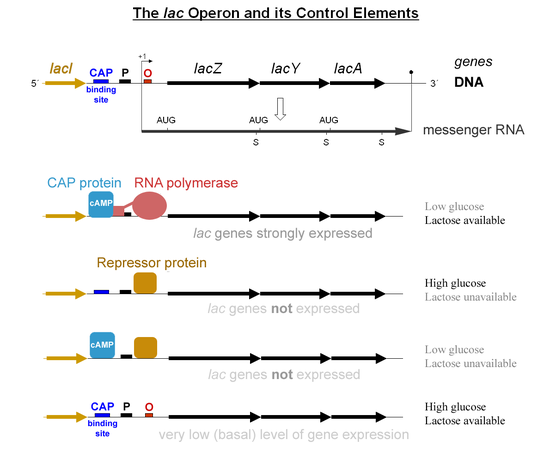
\includegraphics[width=10cm]{con-lac_operon}
  \caption[Example of gene regulation]{\label{fig:con-lac_operon} Example of gene regulation (Lac operon). Retrieved from \url{upload.wikimedia.org/wikipedia/commons/thumb/d/d2/Lac_operon-2010-21-01.png/550px-Lac_operon-2010-21-01.png}}
\end{figure}

\begin{figure}[H]
  \centering
  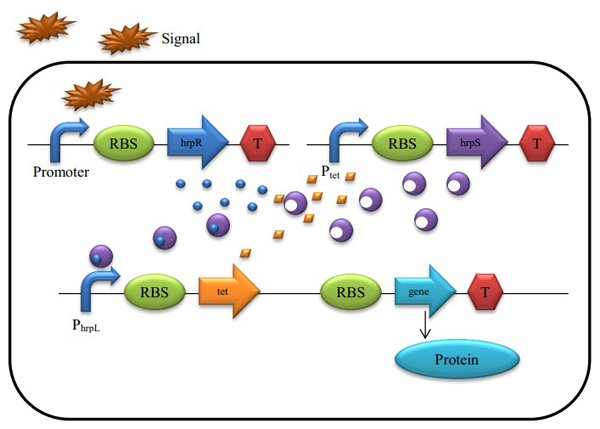
\includegraphics[width=10cm]{con-parts_of_DNA}
  \caption[Parts of a gene]{\label{fig:con-parts_of_DNA} The promoter, RBS, stop codon are shown. Retrieved from \url{http://2013.igem.org/wiki/images/c/c6/HIT-Harbin_Project_Schematic.png}}
\end{figure}

Therefore, in addition to the genotype, gene expression is very important for the cells to develop properly. And, together with the genetic information, defines its structure and behavior. With this in mind, and the fact that those networks may be very large and complex, the approach that Systems Biology is proposing consists on focusing on the interactions between the different genes and components of a cell rather than on the details of the structure of the molecules involved. The set of interactions may be visualized as biological circuits, that are groups of genes that regulate each other's expression. Figure \ref{fig:con-biocircuits_conv} shows some of the conventions used in the schemes of biological circuits.

\begin{figure}[H]
  \centering
  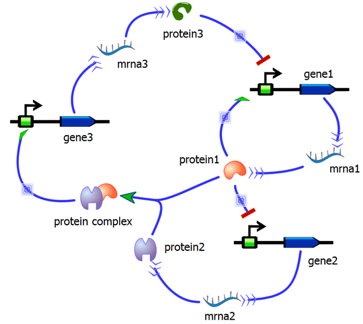
\includegraphics[width=10cm]{con-biocircuits_conv}
  \caption[Systems biology conventions]{\label{fig:con-biocircuits_conv} Typical conventions for biological circuits used in Systems Biology. Retrieved from \url{http://beacon-center.org/wp-content/uploads/2012/10/SyntheticGeneCircuit.png}}
\end{figure}

\begin{figure}[H]
  \centering
  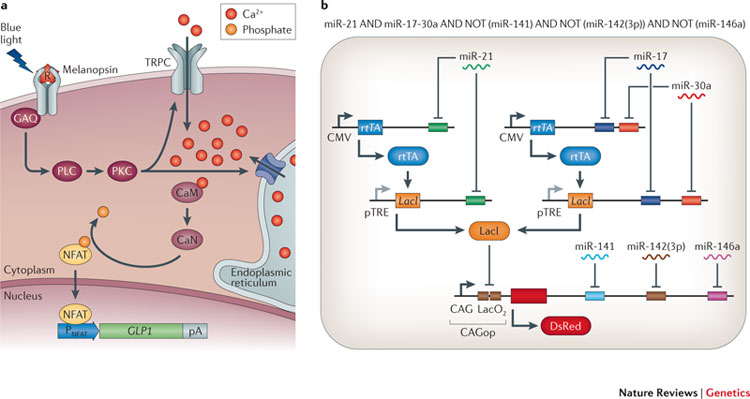
\includegraphics[width=12cm]{con-biocircuits_comp}
  \caption[Example of a biological circuit]{\label{fig:con-biocircuits_comp} Example of a biological circuit. Retrieved from \url{http://www.nature.com/nrg/journal/v13/n6/images/nrg3227-i2.jpg}}
\end{figure}

\section{Hill functions}
\label{sec:hill}

To model the regulation on a gene by a transcription factor, a widely used model is the Hill equation. We will derive it for a particular case that allows a phenomenological understanding of the principles \cite{alon06}.

Consider a transcription factor $X$ that binds to the promoter of some gene, we will label the promoter (gene) as $D$. Also, suppose that $X$ has $n$ binding sites on the promoter and ignore the intermediate states, where less than $n$ molecules of $X$ are bound. The chemical equation is

\begin{equation*}
  \ce{n[X] + [D]} \ce{<=>[k_+][k_-]} \ce{[nXD]}.
\end{equation*}

Hence, $[nXD]$ changes over time as

\begin{equation*}
  \frac{\mathrm{d}[nXD]}{\mathrm{d}t} = k_+[X]^n[D] - k_-[nXD],
\end{equation*}

which in steady state yields

\begin{equation}
  \label{eq:hillss}
  [X]^n[D] = \frac{k_-}{k_+}[nXD].
\end{equation}

Taking the total number $D_T$ of copies of the gene (promoter and DNA molecules) as a constant we obtain

\begin{equation*}
  [D_T] = [D]+[nXD].
\end{equation*}

Solving for the free DNA concentration $[D]$ and replacing in eq. \eqref{eq:hillss}

\begin{equation*}
  [X]^n\left([D_T]-[nXD]\right) = \frac{k_-}{k_+}[nXD].
\end{equation*}

$[nXD]/[D_T]$ and $[D]/[D_T]$ are the fractions of DNA bound and unbound to the transcription factor, respectively, solving for those quantities we obtain

\begin{equation*}
  \frac{[nXD]}{[D_T]} = \frac{[X]^n}{K_d^n+[X]^n}, \quad\quad\quad\quad\quad  \frac{[D]}{[D_T]} = \frac{K_d^n}{K_d^n+[X]^n} = \frac{1}{1+\left(\frac{[X]}{K_d}\right)^n},
\end{equation*}

where $K_d^n \coloneqq k_-/k_+$. In a timescale such that many bindings and unbindings of the transcription factor to the promoter have occurred, those fractions can be interpreted as the probability of having $n$ bound molecules of $X$, and the probability for being unbound, respectively. If the increasing in transcription rate with respect to the basal rate $a$ is proportional to the probabilities of being bound for an activator, and of being unbound for a repressor, the net rates are

\begin{equation}
  \label{eq:con-hillac}
  f([X]) = a + b \frac{[X]^n}{K_d^n+[X]^n},
\end{equation}

for an activator, and

\begin{equation}
  \label{eq:con-hillrep}
  f([X]) = a + b \frac{1}{1+\left(\frac{[X]}{K_d}\right)^n}.
\end{equation}

for a repressor. $b+a$ is the maximum transcription rate, wich happens when $[X]\rightarrow\infty$ for the case of an activator, and when $[X]=0$ for the repressor. $K_d$ is called the \textit{dissociation constant}, which is the concentration of $[X]$ needed for half activation or repression. Biologically it represents the chemical affinity between $x$ and the promoter.  $n$ is called the \textit{Hill coefficient} and from the derivation can be said that it is related to the cooperativity of the transcription factor, being larger if the binding of a molecule of $[X]$ enhances more the binding of another one. A larger value of $n$ give a more step-like Hill function. Figures \ref{fig:con-hill_act} and \ref{fig:con-hill_rep} show the shape of typical Hill functions given by eqs. \eqref{eq:con-hillac} and \eqref{eq:con-hillrep}.

\begin{figure}[H]
  \centering
  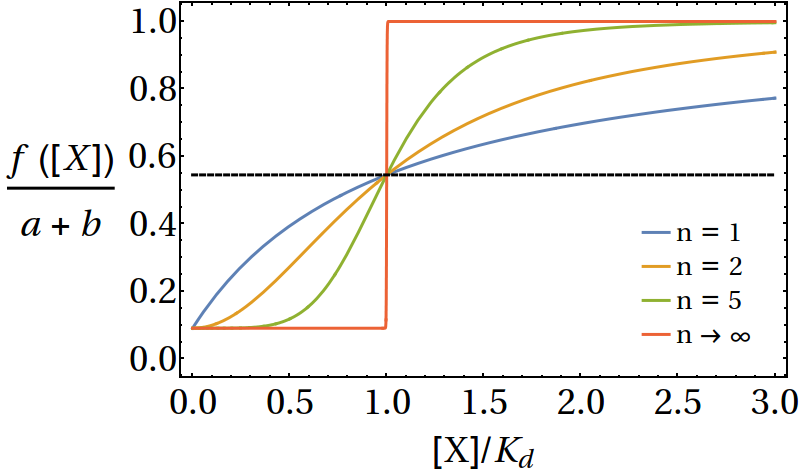
\includegraphics[width=12cm]{con-hill_act}
  \caption[Hill function for an activator]{\label{fig:con-hill_act} Hill functions for an activator. Various values of $n$ are shown. The dashed line shows the point of half activation corresponding to $[X]=K_d$. All have the same value of $K_d$, $a$ and $b$ with $\nicefrac{b}{a}=10$.}
\end{figure}

\begin{figure}[H]
  \centering
  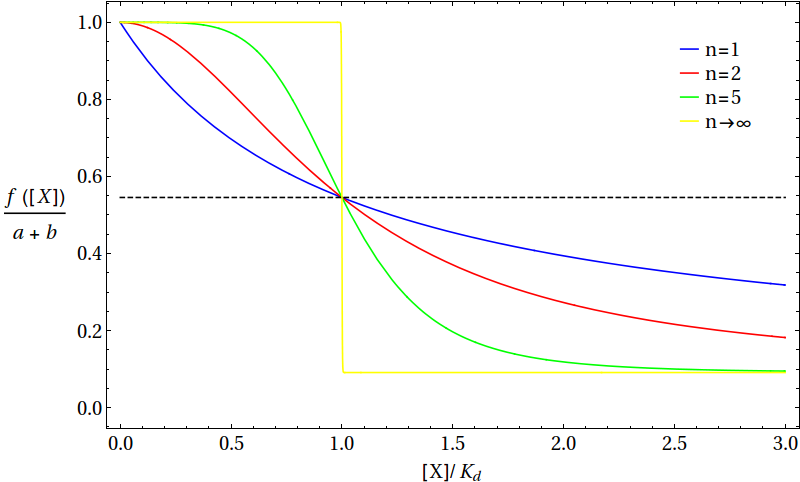
\includegraphics[width=12cm]{con-hill_rep}
  \caption[Hill function for a repressor]{\label{fig:con-hill_rep} Hill functions for a repressor. With the same parameters as fig. \ref{fig:con-hill_act}.}
\end{figure}

Notice in both graphs that as $n\rightarrow\infty$, the function appears more like a Heaviside function with the step in $[X] = K_d$. This approximation can be very useful on a first qualitative analysis of biological circuits but such high values of $n$ are biologically unrealistic. The case $n=1$ corresponds to the Michaelis-Menten equation.

\section{Probability}

Consider an experiment in which the set of possible outcomes is clearly known. A random variable $X$ is a quantity that can take values from that set of possible outcomes $\{x\}$ of the experiment. How likely is that any value $x$ happens in a given trial of the experiment is determined by the probability mass function (PMF) $P(x)$ if the variable is discrete. For a discrete random variable, $P(x)$ represents the fraction of trials of the experiment in which $X$ has the value $x$ when the number of trials is large. The PMFs follow the axioms of nonnegativity, additivity and normalization. \cite{bertsekas08} \footnote{We will focus here on discrete random variables. The continous case is very similar, it reduces almost entirely to change $\sum$ by $\int\mathrm{d}x$ and $P(x)$ by $\rho(x)$, where $\rho(x)$ is the probability density function (PDF), the analogous of the PMF.} 

\todo[inline]{TODO: Explain CDFs?}

For several random variables $X_1,\dotsc,X_n$, the joint PMF  $P(x_1,\dotsc,x_n)$ is defined as the probability that $X_1=x_1,\dotsc,X_n=x_n$. The set of random variables are \textbf{independent} if

\begin{equation*}
  P(x_1,\dotsc,x_n) = P(x_1)\dotsm P(x_n)
\end{equation*}

The conditional probability of the r. v.s $X_1,\dotsc,X_k$ given the variables $X_{k+1},\dotsc,X_n$ is denoted by $P(x_1,\dotsc,x_k|x_{k+1},\dotsc,x_n)$ and it is defined as

\begin{equation*}
  P(x_1,\dotsc,x_k|x_{k+1},\dotsc,x_n) \coloneqq \frac{P(x_1,\dotsc,x_n)}{P(x_{k+1},\dotsc,x_n)},
\end{equation*}

provided that the denominator is different from $0$. It can be thought as the probability of a certain outcome for $x_1,\dotsc,x_k$ when certain given values of $x_{k+1},\dotsc,x_n$ have been obtained. Notice that if all the random variables are independent it reduces to

\begin{equation*}
  P(x_1,\dotsc,x_k|x_{k+1},\dotsc,x_n) = P(x_1,\dotsc,x_k).
\end{equation*}

The conditional and unconditional probabilities are equal, meaning that the outcome of $(x_{k+1},\dotsc,x_n)$ does not affect the outcome of $(x_1,\dotsc,x_k)$.

To find the probability of a certain outcome of $X$, sometimes it is easier to use the \textbf{total probability theorem}

\begin{equation*}
  P(x) = \sum_y P(x,y) = \sum_y P(x|y)P(y).
\end{equation*}

The \textbf{expected value} (also called average) of a function of a random variable $f(X)$ is defined as

\begin{equation}
  \label{eq:con-ave_def}
  \langle f(X)\rangle \coloneqq \sum_xf(x)P(x).
\end{equation}

From the definition can be noticed that the expected value is linear, i.e., for a pair of random variables $X$ and $Y$, and a constant $c$

\begin{equation*}
  \langle X+cY\rangle = \langle X\rangle+c\langle Y\rangle.
\end{equation*}

The variance $\sigma^2(X)$ of $X$ measures the dispersion of the possible outcomes of the random variable, it is defined as

\begin{equation*}
  \sigma^2(X) \coloneqq \left\langle\left( X-\langle X\rangle\right)^2\right\rangle.
\end{equation*}

It can be easily shown that

\begin{equation}
  \label{eq:con-var_nice}
  \sigma^2(X) = \langle X^2\rangle - \langle X\rangle^2.
\end{equation}

From the previous equation it can be seen that for a constant $c$

\begin{equation*}
  \sigma^2(cX) = c^2\sigma^2(X)
\end{equation*}

If $X$ and $Y$ are independent, it can be shown that

\begin{equation}
  \label {eq:con-mom_ind}
  \langle XY\rangle = \langle X\rangle\langle Y\rangle \quad\text{and}\quad \sigma^2(X+Y) = \sigma^2(X)+\sigma^2(Y).
\end{equation}

The conditional expectation of $X$ given a random variable $Y$, $\langle X|Y\rangle$ is itself a random variable which depends on $Y$, which when $Y$ is fixed in some $y$ is given by

\begin{equation*}
  \langle X|y\rangle \coloneqq \sum_xxP(x|y),
\end{equation*}

and it follows that

\begin{equation*}
  \left\langle\langle X|Y\rangle\right\rangle = \left\langle X\right\rangle
\end{equation*}

which is the \textbf{law of total expectation}, for the variance there is an analogous theorem, called the \textbf{law of total variance}

\begin{equation*}
  \sigma^2(x) = \left\langle\sigma^2(x|y)\right\rangle + \sigma^2\left(\langle x|y\rangle\right)
\end{equation*}

The \textbf{covariance} of $X$ and $Y$ is defined as

\begin{equation*}
  \text{cov}(X,Y) \coloneqq \left\langle\left(X-\langle X\rangle\right)\left(Y-\langle Y\rangle\right)\right\rangle = \langle XY\rangle - \langle X\rangle\langle Y\rangle.
\end{equation*}

It can be thought as a measure of how correlated is their behaviour. For example, if the value of $Y$ is known, the value of $X$ will be more likely to be known if the covariance is high in absolute value. The covariance will be $0$ if it does not give us any information. Consider the extreme case, if $Y=X$, $\text{cov}(X,X) = \sigma^2(X)$, while if $X$ and $Y$ are independent by eq. \eqref{eq:con-mom_ind} we get $\text{cov}(X,Y) = 0$.

\section{Noise}
\label{sec:con-noise}
Intuitively, we may expect that a random variable is more 'random' or noisy, when the deviations relative to the expected value are bigger. With this in mind, the noise in a random variable $X$ must increase as the variance increases and decrease as the mean increases (the same deviation from a smaller expected value contributes more to the noise than from a bigger one). The quantities that have benn used to measure noise in biology are the Fano factor $\nu$ and the coefficient of variation $\eta$, which are defined by

\begin{equation}
  \label{eq:con-fano_def}
  \nu_X \coloneqq \frac{\sigma^2(X)}{\langle X \rangle}.
\end{equation}

\begin{equation}
  \label{eq:con-cv_def}
  \eta_X \coloneqq \frac{\sigma(X)}{\langle X \rangle}.
\end{equation}

The Fano factor has been used in the first studies of noise in biology since it had the particular property that for a random variable with a Poisson distribution $\nu_X=1$ and hence it measures deviations from a Poissonian behavior. In more recent studies the coefficient of variation is being used because it is dimensionless and for that reason it does not depend on the units used for the random variable. For this reason, the generic term 'noise' is now used to refer to $\eta$.

\section{Moment generating functions}

Let $n_1,\dotsc,n_N$ be discrete random variables over $\mathbb{N}$ and let $f(n_1,\dotsc,n_N)$ be the joint probability mass function. The moment generating function $F(z_1,\dotsc,z_N)$ is defined as \footnote{Not to be confused with the cumulative distribution function}

\begin{equation}
  \label{def:mom_gen}
  F(z_1,\dotsc,z_N) \coloneqq \sum_{\mathclap{n_1=0}}^{\infty} \dotsi \sum_{\mathclap{n_N=0}}^{\infty} z_1^{n_1} \dotsm z_N^{n_N} f(n_1,\dotsc,n_N).
\end{equation}

Evaluating the function on $z_1 = \dotsb = z_N = 1$ (denoted by $\left. \right|_1$) we obtain

\begin{equation}
  \label{eq:con-mom_gen_1}
  \left.F\right|_1 = \sum_{\mathclap{n_1,\dotsc,n_N}}f(n_1,\dotsc,n_N) = 1.
\end{equation}

by the axiom of normalization. Taking the derivative of eq. \ref{def:mom_gen} with respect to $z_i$, $i = 1,\dotsc,N$ we get

\begin{equation}
  \label{eq:con-mom_gen_d1}
  \left.\frac{\partial F}{\partial z_i}\right|_1 = \left.\sum_{\mathclap{n_1,\dotsc,n_N}}n_i z_1^{n_1}\dotsm z_i^{n_i-1}\dotsm z_N^{n^N}f(n_1,\dotsc,n_N)\right|_1 = \sum_{\mathclap{n_1,\dotsc,n_N}} n_i f(n_1,\dotsc,n_N) = \langle n_i \rangle.
\end{equation}

Differentiating again with respect to $z_j$, $j=1,\dotsc,N$ with $j\neq i$ we obtain

\begin{equation}
  \label{eq:con-mom_gen_d1d2}
  \left. \frac{\partial F}{\partial z_i z_j} \right|_1 = \langle n_i n_j \rangle.
\end{equation}

Differentiating eq. \ref{def:mom_gen} twice with respect to $z_i$ we obtain similarly

\begin{equation}
  \label{eq:con-mom_gen_d1d1}
  \left. \frac{\partial^2F}{\partial z_i^2}\right|_1 = \langle n_i(n_i-1) \rangle.
\end{equation}

These properties will be very useful in the next sections to find the noise of a genetic system.

\section{Characteristic function}
\label{sec:con-charac_func}
Another transformation of the PMF that has properties similar to the mentioned for the moment generating function is the characteristic function. It is defined for a $N$-tuple of random variables $(X_1,\dotsc,X_N)$ as\footnote{We will consider here the case with the real exponent}.

\begin{equation*}
  \phi(s_1,\dotsc,s_N)\coloneqq \left\langle e^{\sum_{i=1}^Ns_ix_i}\right\rangle = \sum_{x_1}\dotsi\sum_{x_N}\exp\left(\sum_{i=1}^Ns_ix_i\right).
\end{equation*}

We will denote the evaluation at $s_1=\dotsb=s_N=0$ by $|_0$ It is easy to see that by normalization

\begin{equation*}
  \phi(s)|_0 = 1.
\end{equation*}

Differentiating once with respect to $s_i$ for $i=1,\dotsc,N$.

\begin{equation}
  \label{eq:con-char_1}
  \left.\frac{\partial\phi(s_1,\dotsc,s_N)}{\partial s_i}\right|_0 = \left.\left\langle x_i e^{\sum_{i=1}^Ns_ix_i}\right\rangle\right|_0 = \langle x_i\rangle.
\end{equation}

Each differentiation with respect to $s_i$ produces a factor $x_i$ in the average, hence

\begin{equation}
  \label{eq:con-char_2}
  \left.\frac{\partial^2\phi(s_1,\dotsc,s_N)}{\partial s_i \partial s_j}\right|_0 = \langle x_ix_j\rangle.
\end{equation}

This equation is valid for any $i,j=1,\dotsc,N$, even for the case $i=j$. In that case the right hand side becomes $\langle x_i^2\rangle$. By calculating higher order derivatives we can find higher order moments in the same way.
  
\section{Stochastic processes}

A stochastic process $X(t)$ \footnote{or $\{X\}_n$ if the time steps are discrete} is a set of random variables indexed by another variable, which usually is taken to be the time. An outcome of the stochastic process is a function of time which varies randomly between different repetitions of the experiment \cite{vankampen92} \cite{gardiner03}.

The \textbf{autocorrelation} $C_X$ of a stochastic process $X(t)$ is given by

\begin{equation*}
  C_X(t,t') \coloneqq \langle X(t)X(t')\rangle.
\end{equation*}

It measures the degree of correlation between outcomes of the random variables at different times. If the process $X$ is \textbf{stationary}, the autocorrelation only depends on the time difference, i.e.

\begin{equation*}
  C(\tau) \coloneqq \langle X(t)X(t+\tau)\rangle,
\end{equation*}

where $\tau \coloneqq t'-t$.

The \textbf{power spectrum} $S_X$ of a stochastic process is defined as average of the square norm of its the Fourier transform

\begin{equation*}
  S_X(\omega) \coloneqq \left|\langle\hat X\rangle\right|^2,
\end{equation*}

where the hat denotes Fourier transform. A mathematical tool that will be very useful in the calculations is the \textbf{Wiener-Khinchin theorem} It states that the power spectrum and the autocorrelation are Fourier-Transform pairs, that is

\begin{equation}
  \label{eq:con-wkth}
  \mathscr{F}(C_X(\tau)) = S_X(\omega),\quad\text{and}\quad \mathscr{F}^{-1}(S_X(\omega)) = C_X(\tau).
\end{equation}

\section{The Poisson process}
\label{sec:poisson}

Many of the processes of creation and destruction that occur in this context are modeled as Poisson processes. For example, the creation and destruction of mRNA and proteins.The Poisson process is a continous-time stochastic process that is used to model arrivals when there is some known arrival rate and when the arrivals at different time intervals are independent.

Mathematically, we define $P(k,\tau)$ as the probability that there are $k\in\mathbb{Z}$ arrivals during a time interval $\tau$ and assume that it is the same for any interval of the same length. We denote by $\lambda$ the arrival rate for the process. The Poisson process satisfy the following properties

\begin{itemize}
  \item  $P(k,\tau)$ is the same for all intervals of length $\tau$.
  \item  The value of $P(k,\tau)$ during some particular interval is independent of other intervals.
  \item $P(k,\tau)$ satisfies the following
    \begin{equation*}
      \begin{split}
        P(0,\tau)=1-\lambda\tau+o_0(\tau),\\
        P(1,\tau)=\lambda\tau+o_1(\tau),\\
        P(k,\tau)=o_k(\tau).\quad\text{for } k>1.
      \end{split}
    \end{equation*}
    
    Where $o_k(\tau)$, $k=0,1,\dotsc$ are functions that become negligible compared to $\tau$ as it becomes small, that is

    \begin{equation*}
      \lim_{\tau\to 0}\frac{o_k(\tau)}{\tau}=0.
    \end{equation*}
\end{itemize}

It can be proven that according to the previous properties, $P(k,\tau)$ is given by

\todo[inline]{Prove it? Is that really true?}

\begin{equation*}
  P(k,\tau) = e^{-\lambda\tau}\frac{(\lambda\tau)^k}{k!},\quad k=0,1,\dotsc
\end{equation*}

which is a Poisson distribution, using the definition for the expected value and variance (eqs. \eqref{eq:con-var_nice} and \eqref{eq:con-ave_def}), letting $N_\tau$ be the number of arrivals during a time interval $\tau$  we get after a little algebra

\begin{equation*}
  \langle N_\tau\rangle = \sigma^2(N_\tau) = \lambda \tau.
\end{equation*}

The average number of arrivals in a time $\tau$ is, as intuitively expected, the arrival rate times the length of the interval. From eqs. \eqref{eq:con-fano_def} and \eqref{eq:con-cv_def}, the noise and Fano factor for $N_\tau$ are

\begin{equation}
  \label{eq:con-poisson_noise}
  \nu(N_\tau) = 1,\quad\quad \eta(N_\tau) = \frac{1}{\sqrt{N_\tau}}.
\end{equation}

This proves what was said on section \ref{sec:con-noise} about the previous use of the Fano factor as the standard measure of noise. From the form of $\eta$ we conclude that if the number of events is large, the Poisson noise is negligible. But for a biological system, for instance, the average number of copies of mRNA of a given gene is of the order of $10$. This makes the effect of noise a significant factor. Also, altought the mean number of proteins is of the order of $1000$, the Poisson noise is negligible, but there is an important contribution of noise coming from the RNA and other sources, as we will see on chapter \ref{ch:master}.

Now we will find the time between events, by now let $t=0$ the time of the last event and let $t=T$ the time of the next event, then

\begin{equation*}
  P(T\leq t) =\int_0^tf_T(t')dt'=1-P(T>t) = 1 - P(0,t) = 1 - e^{-\lambda t}.
\end{equation*}

Differentiating and applying the fundamental theorem of calculus, we get the \textbf{exponential PDF}, which is given by

\begin{equation*}
  \label{eq:con-exp_pdf}
  f_T(t) = \lambda e^{-\lambda t}.
\end{equation*}

Therefore, the time $T$ until the first arrival follows an exponential distribution. 

The exponential distribution is \textbf{memoryless} in the following sense: suppose an arrival happened at time $t'$, therefore, the probability distribution for the remaining time until the next arrival is an exponential with the same rate. \todo[inline]{Explain better, prove it?}. With this in mind, not only the time until the first arrival, but all the interarrival times (the times between arrivals), follow the distribution given by eq. \eqref{eq:con-exp_pdf}.

Suppose we $k$ independent Poisson processes with rates $\lambda_1,\dotsc,\lambda_k$ and we record an arrival each time an arrival occur in either process. This merged process is also a Poisson process with rate $\Lambda\coloneqq\sum_{i=1}^k\lambda_i$. Also, any arrival of the merged process has a probability $\lambda_i/\Lambda$, $i=1,\dotsc,k$ of being an arrival of the $i$th process.

In the models we will consider there might be several creation and destruction events which are Poissonian and independent, for example, the synthesis and degradation of different kinds of RNA and protein, the binding of transcription factors, etc. For these models, we can take advantage of the merging properties of Poisson processes to make efficient and precise simulations.

\section{The Gillespie algorithm}

To simulate the models we will use the Gillespie algorithm \cite{gillespie77} which improves speed a lot with respect to brute-force stochastic algorithms. It is used to simulate simultaneous Poissonian events that occur with a certain rate (probability per unit time), e.g. synthesis and degradation of RNA or proteins, binding of an enzyme to a substrate, etc.

In the brute-force approach we consider a fixed time interval that must be sufficiently small, and for every possible event we sample a random number that depending on the probabilities of the events, will tell us which of the events happened or if nothing happened at that interval. This procedure is repeated for all the intervals. Since time intervals must be small and for each interval we must sample as many random numbers as events, this approach is computationally inefficient.

In the Gillespie algorithm, we take advantage of the mentioned properties of the Poisson process \cite{bertsekas08}. There are not fixed time intervals in this case, a random number is sampled with an exponential distribution whose rate $\Lambda$ is the sum of the rates of the individual processes to find the time of occurence of the next event and another uniform one is sampled to evaluate which of the events occured. Using the properties of the exponential CDF, to sample an exponential random number $X$ with parameter $\Lambda$ from an uniform $U$ between $0$ and $1$ we apply the following equation

\todo[inline]{Prove it?}

\begin{equation}
  X = -\frac{1}{\Lambda}\ln(U).
\end{equation}

The Gillespie algorithm is by far more efficient. First, it does not need to have a fixed small time interval, it finds the time intervals between events. Second, the number of random numbers sampled per time interval in the brute-force approach is equal to the number of events (which can be large), and many of the intervals there will not be an event, while in the Gillespie algorithm only two random numbers are sampled by event and the way in which the time interval is sampled allows to go forward in time in many fewer steps. Finally, a very important aspect is that the Gillespie algorithm is that it is exact, while the precision of the brute-force algorithm depends on how small is the time interval in consideration.
